\documentclass[english,11pt]{article}
\usepackage{tikz}
\usetikzlibrary{decorations.pathreplacing}
\usepackage{amssymb}
\usepackage{amsmath}
\usepackage{tcolorbox}   
\usepackage[notref,notcite,color]{showkeys}

\begin{document}

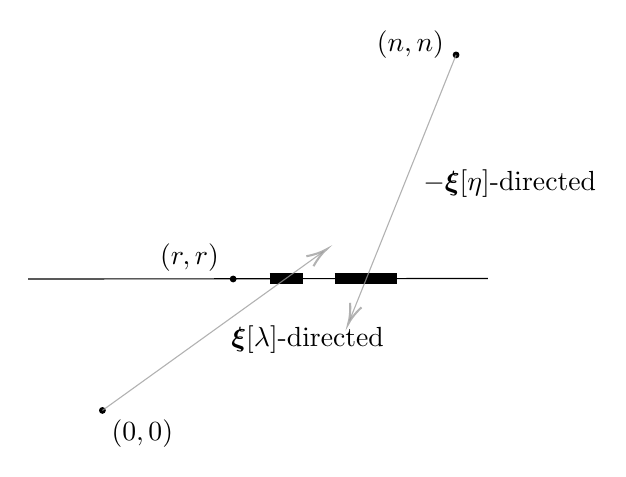
\begin{tikzpicture}[x=0.75pt,y=0.75pt,yscale=-0.9,xscale=0.9]

\draw    (60.32,180.2) -- (306.4,179.88) ;
\draw  [fill={rgb, 255:red, 0; green, 0; blue, 0 }  ,fill opacity=1 ] (98.53,250.54) .. controls (98.53,249.71) and (99.2,249.04) .. (100.03,249.04) .. controls (100.86,249.04) and (101.53,249.71) .. (101.53,250.54) .. controls (101.53,251.37) and (100.86,252.04) .. (100.03,252.04) .. controls (99.2,252.04) and (98.53,251.37) .. (98.53,250.54) -- cycle ;
\draw  [fill={rgb, 255:red, 0; green, 0; blue, 0 }  ,fill opacity=1 ] (287.87,60.21) .. controls (287.87,59.38) and (288.54,58.71) .. (289.37,58.71) .. controls (290.2,58.71) and (290.87,59.38) .. (290.87,60.21) .. controls (290.87,61.04) and (290.2,61.71) .. (289.37,61.71) .. controls (288.54,61.71) and (287.87,61.04) .. (287.87,60.21) -- cycle ;
\draw  [fill={rgb, 255:red, 0; green, 0; blue, 0 }  ,fill opacity=1 ] (168.53,180.17) .. controls (168.53,179.34) and (169.2,178.67) .. (170.03,178.67) .. controls (170.86,178.67) and (171.53,179.34) .. (171.53,180.17) .. controls (171.53,181) and (170.86,181.67) .. (170.03,181.67) .. controls (169.2,181.67) and (168.53,181) .. (168.53,180.17) -- cycle ;
\draw [line width=3.75]    (189.6,179.88) -- (207.6,179.88) ;
\draw [line width=3.75]    (224.4,179.88) -- (258,179.88) ;
\draw [color={rgb, 255:red, 155; green, 155; blue, 155 }  ,draw opacity=0.77 ]   (100.03,250.54) -- (218.38,165.45) ;
\draw [shift={(220,164.28)}, rotate = 144.28] [color={rgb, 255:red, 155; green, 155; blue, 155 }  ,draw opacity=0.77 ][line width=0.75]    (10.93,-3.29) .. controls (6.95,-1.4) and (3.31,-0.3) .. (0,0) .. controls (3.31,0.3) and (6.95,1.4) .. (10.93,3.29)   ;
\draw [color={rgb, 255:red, 155; green, 155; blue, 155 }  ,draw opacity=0.77 ]   (289.37,60.21) -- (232.34,202.42) ;
\draw [shift={(231.6,204.28)}, rotate = 291.85] [color={rgb, 255:red, 155; green, 155; blue, 155 }  ,draw opacity=0.77 ][line width=0.75]    (10.93,-3.29) .. controls (6.95,-1.4) and (3.31,-0.3) .. (0,0) .. controls (3.31,0.3) and (6.95,1.4) .. (10.93,3.29)   ;

% Text Node
\draw (103.53,253.94) node [anchor=north west][inner sep=0.75pt]    {$( 0,0)$};
% Text Node
\draw (129.53,159.67) node [anchor=north west][inner sep=0.75pt]    {$( r,r)$};
% Text Node
\draw (245.53,45.93) node [anchor=north west][inner sep=0.75pt]    {$( n,n)$};
% Text Node
\draw (167.62,203.61) node [anchor=north west][inner sep=0.75pt]    {$\boldsymbol{\xi}[\lambda]$-directed};
% Text Node
\draw (270.42,120.41) node [anchor=north west][inner sep=0.75pt]    {$-\boldsymbol{\xi}[\eta]$-directed};


\end{tikzpicture}

\end{document}